\documentclass{exam}
\usepackage[utf8]{inputenc}
\usepackage{lmodern}
\usepackage{microtype}

% \usepackage[parfill]{parskip}
\usepackage[dvipsnames]{xcolor}
\usepackage{amsmath}
\usepackage{amsfonts}
\usepackage{amsthm}
\usepackage{siunitx}
\DeclareSIUnit\year{yr}
\DeclareSIUnit\foot{ft}
\DeclareSIUnit\litre{\liter}

\usepackage{skull}

\usepackage{pgfplots}
\usepgfplotslibrary{polar}
\pgfplotsset{compat=1.11}
\usepgfplotslibrary{statistics}
\usepackage{graphicx}
\usepackage{sidecap}
\sidecaptionvpos{figure}{c}
\usepackage{float}
\usepackage{gensymb}
\usepackage{tkz-euclide}
\usetkzobj{all}
\usepackage{commath}
\usepackage{hyperref}
\usepackage{enumitem}
\usepackage{wasysym}
\usepackage{multicol}
\usepackage{mathtools}
\usepackage{tcolorbox}
\usepackage{tabularx}
\usepackage[version=4]{mhchem}
\usepackage{changepage}
\usepackage{listings}
\lstset{basicstyle=\ttfamily\linespread{0.8}\small}

\renewcommand*{\thefootnote}{\fnsymbol{footnote}}

\newtheorem*{thm}{Theorem}
\newtheorem*{iden}{Identity}
\newtheorem*{lemma}{Lemma}
\newtheorem{obs}{Observation}
\theoremstyle{definition}
\newtheorem*{defn}{Definition}
\newtheorem*{ex}{Example}
\newtheorem{con}{Construction}
\newtheorem*{alg}{Algorithm}

\newtheoremstyle{break}
  {\topsep}{\topsep}%
  {\itshape}{}%
  {\bfseries}{}%
  {\newline}{}%
\theoremstyle{break}
\newtheorem*{bthm}{Theorem}

% russian integral
\usepackage{scalerel}
\DeclareMathOperator*{\rint}{\scalerel*{\rotatebox{17}{$\!\int\!$}}{\int}}

% \DeclareMathOperator*{\rint}{\int}

\pgfplotsset{vasymptote/.style={
    before end axis/.append code={
        \draw[densely dashed] ({rel axis cs:0,0} -| {axis cs:#1,0})
        -- ({rel axis cs:0,1} -| {axis cs:#1,0});
    }
}}

% \pointsinrightmargin
\boxedpoints
\pointname{}

\newcommand{\questioA}{\question[\texttt{\textbf{\color{Cerulean} A}}]}
\newcommand{\questioM}{\question[\texttt{\textbf{\color{PineGreen} M}}]}
\newcommand{\questioE}{\question[\texttt{\textbf{\color{WildStrawberry} E}}]}
\newcommand{\questioS}{\question[\texttt{\textbf{\color{Goldenrod} S}}]}
\newcommand{\questioO}{\question[\texttt{\textbf{\color{BurntOrange} O}}]}

\newcommand{\parA}{\part[\texttt{\textbf{\color{Cerulean} A}}]}
\newcommand{\parM}{\part[\texttt{\textbf{\color{PineGreen} M}}]}
\newcommand{\parE}{\part[\texttt{\textbf{\color{WildStrawberry} E}}]}
\newcommand{\parS}{\part[\texttt{\textbf{\color{Goldenrod} S}}]}
\newcommand{\parO}{\part[\texttt{\textbf{\color{BurntOrange} O}}]}

\newcommand{\subparA}{\subpart[\texttt{\textbf{\color{Cerulean} A}}]}
\newcommand{\subparM}{\subpart[\texttt{\textbf{\color{PineGreen} M}}]}
\newcommand{\subparE}{\subpart[\texttt{\textbf{\color{WildStrawberry} E}}]}
\newcommand{\subparS}{\subpart[\texttt{\textbf{\color{Goldenrod} S}}]}
\newcommand{\subparO}{\subpart[\texttt{\textbf{\color{BurntOrange} O}}]}

\newcommand{\mainHeader}[2]{\section*{NCEA Level 2 Mathematics\\#1. #2}}
\newcommand{\mainHeaderHw}[2]{\section*{NCEA Level 2 Mathematics (Homework)\\#1. #2}}
\newcommand{\seealso}[1]{\begin{center}\emph{See also #1.}\end{center}}
\newcommand{\drills}[1]{\begin{center}\emph{Drill problems: #1.}\end{center}}
\newcommand{\basedon}[1]{\begin{center}\emph{Notes largely based on #1.}\end{center}}


\begin{document}

\mainHeader{20}{Sampling}
Last time, we mainly looked at the broad picture: what we need to think about, in general, when we try to
answer a statistical question. This time we will begin to think about some of the practical issues we need
to overcome.

As we've already discussed, it is usually impractical to measure an entire population. Our goal is therefore
to measure a smaller sample and then extrapolate our findings. This process, known as \emph{statistical inference},
requires us to have a good method for choosing our sample so that it is representative.

\begin{center}
  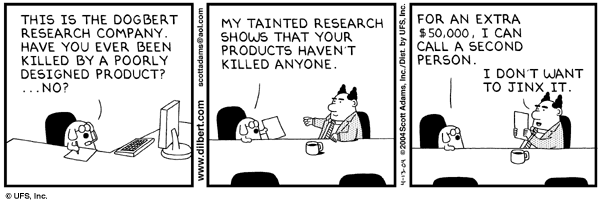
\includegraphics[width=0.8\textwidth]{dilbert-sampling}
\end{center}


We will look at several examples of bad methods of sampling to begin with.

\subsection*{The examples}
\begin{enumerate}
  \item I asked all my friends whether they own a car, and none of them do.
  \item A survey of high-school students samples all the Y13 students at a particular school, and concludes that only
        7\% of students use illegal drugs.
  \item In 1936, a US presidential election poll posted questionnaires to ten million people selected from telephone
        books and club membership lists, and got 2.4 million responses. Based on these, they predicted a decisive
        victory for one candidate (57\% of the popular vote). In reality, the other candidate won by a landslide (62\%).\footnote{Freedman et al., \emph{Statistics}. Section 19.2.}
  \item A psychiatrist finds that practically everyone is neurotic.
  \item A drug trial is performed; the patients were analysed according to the treatment they actually took, rather
        than the treatment they were assigned at the randomisation stage of the trial.
  \item A majority of people attending a public meeting on a new cycleway are strongly against it. However, a combination of online
        survey, door knocking surveys, and paper surveys performed by the council found that 75\% of the population of the area was
        either in favour or strongly in favour of the new cycleway.
  \item The council conducted a survey on a new residential development. The survey was conducted by posting a survey to all those on the list of
        a local resident's association. 90\% of respondents were against the new development.
\end{enumerate}

\subsection*{The problems}
\begin{enumerate}
  \item Some people aren't my friends. In addition, most of my friends live in urban areas with frequent public transport,
        and tend to be more affluent.
  \item This doesn't include students who drop out of school, or are homeschooled. It also only measures students at
        a particular school, which might be more or less affluent than average and thus drug use by its students might be more or less
        probable.
  \item Despite the large sample size, the sampling method used tended to screen out the poor (who didn't belong to clubs, or
        have telephones) who were more likely to vote for the other candidate.
  \item The psychiatrist's patients are far from a sample of the population.
  \item This might seem reasonable (if 30\% of participants drop out, they didn't receive the benefit of the treatment and so
        shouldn't be part of the `participated in treatment' group during analysis). However, the problem is that the question
        that should be being answered is `is this treatment effective?' rather than `out of the people who chose to take our
        tablets, is the treatment effective?'. After all, if people don't end up taking the medication after being given it,
        this is philosophically and medically the same as if the medication was ineffective.\footnote{See Ben Goldacre, \emph{Bad Pharma}, pages 200-1.}
  \item There is a bias in the sample of people attending the public meeting: for example, they are likely to have strong opinions on the cycleway and
        are likely to be more involved in local politics and resident groups. The council survey reaches a broader spectrum of residents and thus
        has less selection bias.
  \item By now, you should be able to come up with your own explanation as to why this sample was not representative.
\end{enumerate}

From studying these examples, we have the following broad guidelines:
\begin{itemize}
  \item When a selection procedure is biased, taking a larger sample with the same bias doesn't help.
  \item If a large proportion of people don't respond, the results are likely to be biased.
  \item Picking a sample from a certain group of people within a population is likely to be biased.
  \item Allowing people to choose whether or not to respond introduces bias.
\end{itemize}

There are various methods of producing a sample, based on these lessons. They include:
\begin{description}
  \item[Simple random sampling] \hfill \\
    Taking a full list of all the people in the population, and picking some proportion of them entirely at random.
  \item[Quota sampling] \hfill \\
    Giving each interviewer a quota of subjects to interview, and interviewing a fixed proportion of particular categories
    within that quota (e.g. 50\% non-male, 20\% below the age of thirty, and so forth) which match the proportion of the
    categories in the overall population.
\end{description}

In general, simple random sampling is the best method as long as it is carried out correctly:
\begin{itemize}
  \item The list of possible interviewees must be a full list of the entire population to be surveyed.
  \item The sampling method should be truly random (in other words, `choosing every $ n$th person' is not a good idea).
\end{itemize}

The problem of non-response bias remains; it is therefore a very good idea to conduct surveys using many different
methods (postal surveys, physical meetings, door-knocking, phone surveys, and so forth) in order to minimise this.

\subsection*{Questions}
\begin{questions}
  \question For each of the following situations, discuss whether or not the sampling plan is `good statistics.'
    \begin{parts}
      \part A restaurant leaves comment cards on all of its tables to encourage diners to participate in a brief survey to learn
            about their overall experience.
      \part A school wants feedback on tuck shop options. Each student has a student identification number; the deans use a computer to
            generate fifty random identification numbers and those students are asked to take a survey.
      \part A council wants feedback on a proposal for new play equipment at a park. They send someone out to stand in the park and
            interview everyone who shows up for five hours one day.
      \part A local company is losing business to the internet; they interview their remaining customers to ask what other services
            that they could provide to draw people in.
      \part A physicist is measuring the power output of a lamp. She makes ten measurements. After entering them into her spreadsheet,
            she finds that a couple are much lower than she would expect, and throws them out.
      \part A student is interested in whether the number of days a year a fellow student cycles to school is correlated with
            the average income of people in the area in which they live. (This data is freely available from the NZ census, and
            is reliable.) They interview fifty students at their school (randomly chosen from the quad one lunchtime), asking them
            roughly how many times they cycled to school in the last year, and which street they live on.
    \end{parts}
  \question Come up with a good sampling plan for the following research questions.
    \begin{parts}
      \part You want to predict the outcome of the upcoming local mayoral election.
      \part You want to know whether people who cycle to school tend to live in `richer' areas.
      \part You want to compare the voting preferences of below-the-voting-age high-schoolers with those
            of the general voting population.
      \part You want to know whether students living in cities are more or less worried about `sustainability'
            than high school students in the country.
      \part You want to know whether or not a cycleway would be generally approved of on a particular stretch of road.
    \end{parts}
\end{questions}

\end{document}

